When designing and implementing machine learning models, scientists act on experience when it comes to architectural decisions and hyperparameter choices. In the early stages of a model, a trained eye on processing examples and observing the loss curve enable rapid progress. However, as the model matures, it becomes essential to quantify its performance with respect to comprehensive validation and test sets. Besides the selection of appropriate validation and test data, it is important to choose a meaningful metric that fits the problem. For example, when all of a models predictions are equally relevant, one would aim for an overall high precision, whereas a use case that involves a human processing the results manually, such as a web search, for example, one would choose a ranking metric that rewards good results at the top of a list.

All considered metrics are defined by terms from the so-called confusion matrix shown in Figure~\ref{fig:2_basics/4_metrics/1_confusion_matrix}. The matrix applies to the general scenario in which predictions are made about a certain condition for a set of objects. Thereby, an object's actual condition can be positive or negative, also referred to as its \emph{ground truth}, as can be the object's predicted condition. A prediction is \emph{true}, or correct, if its predicted condition is consistent with the object's actual condition and \emph{false} otherwise. Furthermore, objects whose prediction is positive are called \emph{positives}, while objects whose predictions are negative are called \emph{negatives}. Depending on their actual and their predicted condition, each object falls into one of four distinct categories:

\begin{figure}[t]
    \centering
    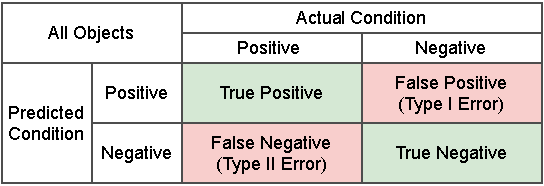
\includegraphics[width=\textwidth]{2_basics/4_metrics/confusion_matrix}
    \caption{Confusion Matrix dividing objects into four distinctive groups depending on their actual and predicted condition}
    \label{fig:2_basics/4_metrics/1_confusion_matrix}
\end{figure}

\begin{itemize}
    \item \textbf{\emph{True positives}} (TP) are objects for which the regarded condition is positive and whose predicted conditions is also positive.

    \item \textbf{\emph{False positives}} (FP) are objects for which the regarded condition is positive but whose predicted condition is negative. This type of error is referred to as a \emph{Type I error}.

    \item \textbf{\emph{False negatives}} (FN) are objects for which the condition is actually negative but whose predicted condition is positive. This second kind of errornous prediction is also referred to as \emph{Type II error}.

    \item \textbf{\emph{True negatives}} (TN) are objects for which the condition is actually negative and whose predicted condition is also negative.
\end{itemize}

Although it is generally desirable to obtain as many correct predictions as possible, true positives and true negatives are often differently important and errors of type one and two differently severe. In medicine, for example, not recognizing a disease could be much worse than accidentally diagnosing a healthy person as ill. Conversely, not recognizing guilt in a lawsuit might be less serious than convicting someone who is innocent. In the context of knowledge graph completion under the open-world assumption, the focus lies on true positives since the KGC model cannot make any qualified statements about false facts without negative samples in the graph. Omitting a fact from the prediction only means that the model has too little evidence for that fact, not that it can falsify it.

%The purpose of this section is to explain those metrics relevant for this work. Section~\ref{fig:2_basics/4_metrics/1_confusion_matrix} defines basic terms used by the following sections. Sections~\ref{subsec:2_basics/4_metrics/2_accuracy} and~\ref{subsec:2_basics/4_metrics/3_prf} then present the general purpose metrics accuracy, precision, recall and F1 score while Sections~\ref{subsec:2_basics/4_metrics/4_mrr} and~\ref{subsec:2_basics/4_metrics/5_map} discuss the ranking metrics MRR and mAP\@.

%\subsection{Confusion Matrix}
%\label{subsec:2_basics/4_metrics/1_confusion_matrix}
%All considered metrics are defined with the help of terms from a so-called confusion matrix as shown in Figure~\ref{fig:3_basics/4_metrics/1_confusion_matrix}. The matrix emerges from the general scenario in which predictions are made for a set of objects that can be either true or false. A prediction is true if its statement is consistent with reality about the object, also called ground truth, and false if the prediction contradicts reality. An example scenario would be an image recognition that has to determine whether a photo shows a cat or not. Then, four mutually exclusive types of predictions can be distinguished:

\begin{itemize}
    \item \textbf{\emph{True positives}} (TP) are predictions stating that a condition holds true when this is indeed the case. In the image recognition example, this would correspond to the case where the model correctly classifies a cat image as a cat.

    \item \textbf{\emph{False positives}} (FP) are negative predictions about objects where the condition is actually true, e.g. declaring an animal as cat although it is not. This type of error is also referred to as a \emph{Type 1 error}.

    \item \textbf{\emph{False negatives}} (FN) are another kind of erroneous predictions, also referred to as \emph{Type 2 errors}. They represent the case that an element with a true condition was classified as false - was overlooked, so to speak. An example would be a cat image not recognized as a cat.

    \item \textbf{\emph{True negatives}} (TN) are similar to true positives in that they are correct predictions, as well. They consist of rejective predictions about objects where the condition does indeed not apply, for example by recognizing that there is no cat in a cat-less photo.
\end{itemize}

Although it is generally desirable to obtain as many correct predictions as possible, true positives and negates are often differently important and errors of type one and two differently severe. In medicine, for example, not recognizing a disease could be much worse than accidentally diagnosing a healthy person as ill. Conversely, not recognizing guilt in a lawsuit might be less serious than convicting someone who is innocent. In the context of knowledge graph completion under the open-world assumption, the focus lies on true positives since the KGC model cannot make any qualified statements about non-applying facts without negative samples in the graph. Omitting a fact from the prediction only means that the model has too little evidence for that fact, not that it can falsify it.

\begin{figure}[t]
    \centering
    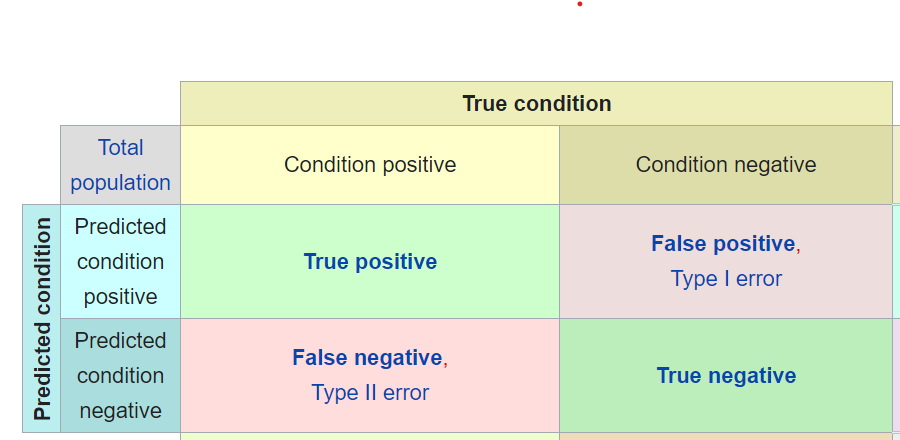
\includegraphics[width=\textwidth]{3_basics/4_metrics/1_confusion_matrix/matrix}
    \caption{Confusion Matrix}
    \label{fig:3_basics/4_metrics/1_confusion_matrix}
\end{figure}

"positive", "negative", "true", "false" predictions, "positive", "negative" elements

cat example
ir scenario


\subsection{Accuracy}
\label{subsec:2_basics/4_metrics/2_accuracy}
One of the most common general-purpose metrics is \emph{accuracy}, which measures a model's overall capability to make correct positive and negative predictions. In the case of binary classification, accuracy is the rate of correct predictions over all predictions:

\begin{align}
    Accuracy = \frac{TP + TN}{TP + TN + FP + FN}
    \label{eq:2_basics/2_metrics/1_accuracy/accuracy}
\end{align}

Colloquially speaking, accuracy answers the question of how good predictions are in general. It takes values in $[0, 1]$, whereby higher is better. However, although accuracy is a useful and intuitive metric in general, it can be misleading when it comes to unbalanced classes because a model can simply reach high accuracy by always predicting the predominant class. For example, if nine out of ten ground truth values are false, a model could reach 90\% accuracy by always predicting false. To counteract this, balanced accuracy~\cite{Mower2005PREPMtPR} can be used instead. However, as mention earlier, as negative predictions do not play a big role for KGC models in an open-world scenario, accuracy will only play a minor role in this work.


\subsection{Precision, Recall and F1}
\label{subsec:2_basics/4_metrics/3_prf}
\emph{Precision}, \emph{recall} and \emph{F1} focus on positive predictions. Precision gives an impression of how reliable positive predictions are, recall tells how many of the actual positive elements are declared as such, and F1 is a measure that combines both precision and recall in one value. All three metrics take values from $[0, 1]$ whereby higher is better.

Precision, also known as \emph{positive predictive value (PPV)}, is the ratio of true positive predictions to all positive predictions as noted in \autoref{eq:2_basics/2_metrics/2_prf/precision}. False negatives are not considered. If a model does not produce any predictions, precision is undefined and has to be defined in accordance with the evaluation scenario. One possibility is to define as 1 if the dataset does not contain any ground truth positives and 0 otherwise, because the model should not produce any predictions if, and only if, there are no ground truth positives.

\begin{align}
    Precision = \frac{TP}{TP + FP}
    \label{eq:2_basics/2_metrics/2_prf/precision}
\end{align}

Recall, on the other hand, also known as \emph{true positive rate (TPR)}, compares the number of true positives to the number of all ground truth positives as shown in \autoref{eq:2_basics/2_metrics/2_prf/recall}. False positives do not count in. If the evaluated dataset does not contain any ground truth positives, recall is undefined and might be specified as 1, because the model did not miss out on any ground truth positives.

\begin{align}
    Recall = \frac{TP}{TP + FN}
    \label{eq:2_basics/2_metrics/2_prf/recall}
\end{align}

Precision and recall are directly dependent on each other. A cautious model that only predicts positives when it is sure achieves high precision but low recall. Conversely, it is easy to achieve optimal recall by making positive predictions for all elements, though precision will suffer in that case. The \emph{F score} serves as a measure that considers both goals and reaches a high value when a reasonable balance between precision and recall is found. \autoref{eq:2_basics/2_metrics/2_prf/f_beta} shows the formula for the general $F_\beta$ score whose parameter $\beta$ determines whether the focus should rather be shifted towards precision or recall. Setting $\beta = 1$ yields the $F_1$ score in \autoref{eq:2_basics/2_metrics/2_prf/f_1} as the harmonic mean in which precision and recall are weighted equally.

\begin{align}
    F_\beta &= (1 + \beta^2) \cdot \frac{Precision \cdot Recall}{\beta^2 \cdot Precision + Recall}
    \label{eq:2_basics/2_metrics/2_prf/f_beta} \\
    F_1 &= 2 \cdot \frac{Precision \cdot Recall}{Precision + Recall}
    \label{eq:2_basics/2_metrics/2_prf/f_1}
\end{align}

Oftentimes, the predictions that should be made for a set of objects can be divided into subsets. For example, in a multi-label classification scenario, metrics can be calculated class-wise and when predicting facts for a set of entities, metrics can be calculated for each entity. In these cases there are multiple ways to calculate the metrics for the overall dataset:

\begin{itemize}
    \item Throw all predictions together and calculate the metrics over all predictions. This approach yields so-called \emph{micro} metrics, for example, micro precision.

    \item Calculate the metrics per subset, for example, class-wise, and specify the resulting values as such. This approach can yield detailed insights but potentially leads to many key figures.

    \item Calculate the metrics per subset and average the results, yielding \emph{macro} metrics.
\end{itemize}


\subsection{Mean Reciprocal Rank}
\label{subsec:2_basics/4_metrics/4_mrr}
The above presented accuracy, precision, recall and F1 metrics are useful in a classification task where no prioritization among the predictions is required. However, in an \emph{information retrieval (IR)} scenario, such as a web search, for example, a model might yield a sorted list of predictions where the ranking actually plays a major role. Usually, IR scenarios do not differentiate between positive and negative predictions, but rather between more or less relevant predictions that are returned by decreasing relevance.

In those cases it is more important to rank relevant items as high as possible among the overall results than it is assign the correct probability, or class if there is probability threshold, to each item. When it is most important to receive a correct top-most prediction for each query, the \emph{mean reciprocal rank (MRR)} is the metric of choice. Given the results of $n$ queries it is calculated as per \autoref{subsec:2_basics/2_metrics/3_mrr}, where $rank_i$ is the rank of the top-most relevant item among the predictions of the $i$th query results. Each reciprocal rank, and thus the mean over all reciprocal ranks, lies in $(0, 1]$, with higher being better. If a query result does not contain any relevant item, the reciprocal rank is undefined. Depending on the use case, the object might be skipped or assigned a specific value. A typical application scenario for MRR would be the evaluation of a voice assistant that has to respond with the single most relevant answer it gets from a model.

\begin{align}
    MRR = \frac{1}{n} \sum_{i=1}^{n} \frac{1}{rank_i}
    \label{eq:2_basics/2_metrics/3_mrr/mrr}
\end{align}


\subsection{Mean Average Precision}
\label{subsec:2_basics/4_metrics/5_map}
Another metrics that considers ranking is \emph{average precision (AP)}. In contrast to MRR it considers not only the top-most relevant result, but all of relevant results, including those not retrieved if the results are limited to a certain number. Given an object for which there are a set of relevant items $R$ and a model that predicts a set of items $P$, average precision is calculated as per Equation~\ref{eq:2_basics/4_metrics/5_map/ap}, in which $Prec@k$ is the precision among the first $k$ retrieved items and $rel@k$ is 1 if the $k$th item is relevant and 0 otherwise.

\begin{align}
    AP = \frac{1}{|R|} \sum_{k=1}^{|P|} Precision@k \cdot rel@k
    \label{eq:2_basics/4_metrics/5_map/ap}
\end{align}

Figure~\ref{fig:2_basics/4_metrics/4_mrr/mrr_map} illustrates the calculation of average precision by an example modeled after a possible list of facts predicted by the Power model when applied to the example entity Lisa from the graph in Chapter~\ref{ch:1_introduction}. Given the list of four predicted facts, sorted by confidence and covering two relevant facts, average precision for Lisa is calculated by adding up the $Precision@k$ values of the relevant facts and dividing the sum by the total number of relevant facts, including the one missing from the predictions.

\begin{figure}[t]
    \centering
    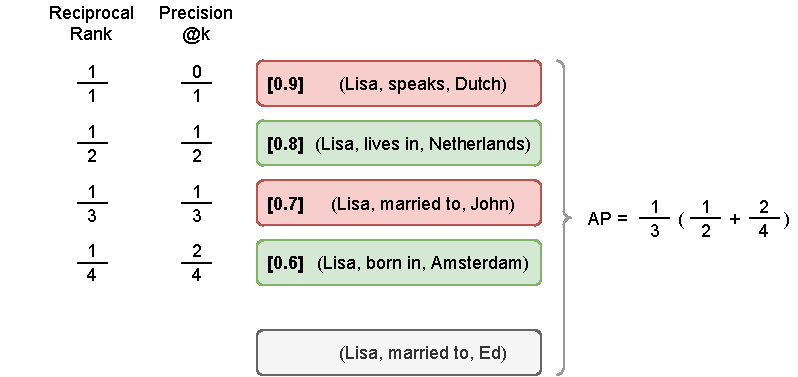
\includegraphics{2_basics/4_metrics/5_map/mrr_map}
    \caption{Calculation of average precision by example of a list of fact predictions, ranked by confidence and containing two of the totally three relevant facts - relevant facts are in green, irrelevant ones in red and the missed out relevant one in grey}
    \label{fig:2_basics/4_metrics/5_map/mrr_map}
\end{figure}

As for the MRR, mAP takes values in $(0, 1]$ and is not defined if there are no relevant items for an object. Again, the latter case might be handled by ignoring such objects. When evaluating $n$ objects, each with $AP_i$ with $1 <= i <= n$, \emph{mean average precision (mAP)} is calculated as the overall average value:

\begin{align}
    mAP = \frac{1}{n} \sum_{i=1}^{n} AP_i
    \label{eq:2_basics/4_metrics/5_map/map}
\end{align}



